\documentclass[
  11pt,
  twocolumn,
  a4paper,
%  bibliography=totoc,     % Literatur im Inhaltsverzeichnis
]{article}


% Paket float verbessern
\usepackage{scrhack}

% Warnung, falls nochmal kompiliert werden muss
\usepackage[aux]{rerunfilecheck}

% unverzichtbare Mathe-Befehle
\usepackage{amsmath}
% viele Mathe-Symbole
\usepackage{amssymb}
% Erweiterungen für amsmath
\usepackage{mathtools}
% Fonteinstellungen
\usepackage{fontspec}
% Latin Modern Fonts werden automatisch geladen
% Alternativ zum Beispiel:
%\setromanfont{Libertinus Serif}
%\setsansfont{Libertinus Sans}
%\setmonofont{Libertinus Mono}

% Wenn man andere Schriftarten gesetzt hat,
% sollte man das Seiten-Layout neu berechnen lassen
% \recalctypearea{}
% deutsche Spracheinstellungen
\usepackage{polyglossia}
\setmainlanguage{german}

\usepackage{marvosym}
\usepackage[
  math-style=ISO,    % ┐
  bold-style=ISO,    % │
  sans-style=italic, % │ ISO-Standard folgen
  nabla=upright,     % │
  partial=upright,   % ┘
  warnings-off={           % ┐
    mathtools-colon,       % │ unnötige Warnungen ausschalten
    mathtools-overbracket, % │
  },                       % ┘
]{unicode-math}

% traditionelle Fonts für Mathematik
\setmathfont{Latin Modern Math}
% Alternativ zum Beispiel:
%\setmathfont{Libertinus Math}

\setmathfont{XITS Math}[range={scr, bfscr}]
\setmathfont{XITS Math}[range={cal, bfcal}, StylisticSet=1]

% Zahlen und Einheiten
\usepackage[
  locale=DE,                   % deutsche Einstellungen
  separate-uncertainty=true,   % immer Fehler mit \pm
  per-mode=symbol-or-fraction,
  alsoload=hep,                % / in inline math, fraction in display math
]{siunitx}
\sisetup{math-micro=\text{µ},text-micro=µ}
\DeclareSIUnit\micron{\micro\metre}
\DeclareSIUnit\mrad{\milli\rad}
\DeclareSIUnit\gauss{G}
\DeclareSIUnit\eVperc{\eV\per\clight}
\DeclareSIUnit\nanobarn{\nano\barn}
\DeclareSIUnit\picobarn{\pico\barn}
\DeclareSIUnit\femtobarn{\femto\barn}
\DeclareSIUnit\attobarn{\atto\barn}
\DeclareSIUnit\zeptobarn{\zepto\barn}
\DeclareSIUnit\yoctobarn{\yocto\barn}
\DeclareSIUnit\nb{\nano\barn}
\DeclareSIUnit\pb{\pico\barn}
\DeclareSIUnit\fb{\femto\barn}
\DeclareSIUnit\ab{\atto\barn}
\DeclareSIUnit\zb{\zepto\barn}
\DeclareSIUnit\yb{\yocto\barn}

% chemische Formeln
\usepackage[
  version=4,
  math-greek=default, % ┐ mit unicode-math zusammenarbeiten
  text-greek=default, % ┘
]{mhchem}

% richtige Anführungszeichen
\usepackage[autostyle]{csquotes}

% schöne Brüche im Text
\usepackage{xfrac}

% Standardplatzierung für Floats einstellen
\usepackage{float}
\floatplacement{figure}{htbp}
\floatplacement{table}{htbp}

\RequirePackage{luatex85}
\usepackage[
  locale=DE,
]{siunitx}

\usepackage{tikz}
\usepackage[
  europeanresistors, % follow DIN
  americaninductors, % follow DIN
  siunitx,
]{circuitikz}
\usepackage{stackengine}
\AtBeginDocument{
  \sisetup{
    math-rm=\mathrm,
    math-micro=µ, % AltGr+m = MICRO SIGN, Unicode: U+00B5
  }
}

% Floats innerhalb einer Section halten
\usepackage[
  section, % Floats innerhalb der Section halten
  below,   % unterhalb der Section aber auf der selben Seite ist ok
]{placeins}

% Seite drehen für breite Tabellen: landscape Umgebung
\usepackage{pdflscape}

% Captions schöner machen.
\usepackage[
  labelfont=bf,        % Tabelle x: Abbildung y: ist jetzt fett
  font=small,          % Schrift etwas kleiner als Dokument
  width=0.9\textwidth, % maximale Breite einer Caption schmaler
]{caption}
% subfigure, subtable, subref
\usepackage{subcaption}

% Grafiken können eingebunden werden
\usepackage{graphicx}
% größere Variation von Dateinamen möglich
\usepackage{grffile}

% schöne Tabellen
\usepackage{booktabs}

% Verbesserungen am Schriftbild
\usepackage{microtype}

% Literaturverzeichnis
\usepackage[
  backend=biber,
]{biblatex}
% Quellendatenbank
\addbibresource{lit.bib}
\addbibresource{programme.bib}

% Hyperlinks im Dokument
\usepackage[
  unicode,        % Unicode in PDF-Attributen erlauben
  pdfusetitle,    % Titel, Autoren und Datum als PDF-Attribute
  pdfcreator={},  % ┐ PDF-Attribute säubern
  pdfproducer={}, % ┘
]{hyperref}
% erweiterte Bookmarks im PDF
\usepackage{bookmark}

% Trennung von Wörtern mit Strichen
\usepackage[shortcuts]{extdash}

%Multirow Einbindung
\usepackage{multirow}

%rotating Einbindung
\usepackage{rotating}

%noindent immer da


% \documentclass[11pt, twocolumn, a4paper]{article}

\setlength{\oddsidemargin}{0.0 cm}
\setlength{\evensidemargin}{0.0 cm}
\setlength{\topmargin}{-1cm}
\setlength{\textheight}{24 cm}
\setlength{\textwidth}{16 cm}

\pagestyle{plain}

\setlength{\parindent}{0in}

\begin{document}

\author{Nils Breer}
\date{Technische Universit\"at Dortmund}

\title{Proceeding to the LHC seminar talk \textit{Update of the $B^0$ \to $K^{*0}$ µ$^{+}$ µ$^{-}$ angular analysis at LHCb} held by Eluned Smith on behalf of the LHC collaboration on 13th of March 2020.}

\maketitle

% hier kommt ein abstract rein!!

The stated Process is of such importance because the
$b \to s \mu \mu$ transition is forbidden at tree level due to FCNC and can only occur at loop order.
Because of that, these processes are much more sensitive to new physics(NP).

\begin{figure}[htb]
  \centering
  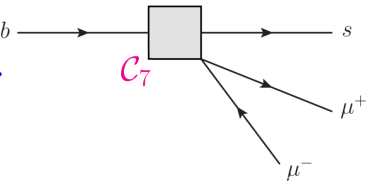
\includegraphics[width=0.5\textwidth]{flavor_plots/wilson_c7.png}
  \caption{Wilson coefficient $C_7$ in .}
  \label{fig:sm_process}
\end{figure}

\begin{figure}[htb]
  \centering
  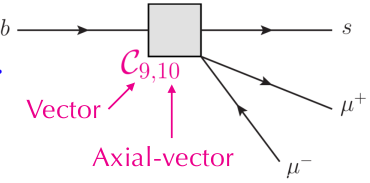
\includegraphics[width=0.5\textwidth]{flavor_plots/wilson_c9_c10.png}
  \caption{Process in new physics model.}
  \label{fig:np_process}
\end{figure}

To gather information about short distance NP above the SM energy scale $\mu$, wilson coefficients $C_i(\mu)$ and low-energy QCD Operators $O_i$ are used to describe that.

The wilson coefficients $C_7$, $C_9$ and $C_{10}$ are of great importance since observables like the forward-backward asymmetry and $P_5\prime$ are sensitive for $C_9$ especially.

In an effective theory, $C_9$ and $C_{10}$ are used to describe the contribution from loops, in which electroweak gauge bosons are produced.  wilson coefficient $C_7$ describes the contribution from loopdiagramms which produce photons from the loops.

This can be summarized by an effective hamiltonian
\begin{equation*}
  H_{eff} = - \frac{4 G_f}{\sqrt{2}} \symup{V}_{tb} \symup{V}_{ts}^{*} \sum_i
  C_i \cdot O_i + \text{h.c.}
\end{equation*}

$G_F$ is Fermi's constant, $\mu$ ist the renormalization scale, $\symup{V}_{tb} \symup{V}_ts^{*}$ is the contains leading flavor factors of the SM which lie in the CKM matrix elements $V_{ij}$

% \section{angular Analysis}
To measure the decay rate as a function of angles of the decay products, an angular analysis is performed.
The definition of the angular observables $\theta_{k}$, $\theta_{l}$ and $\phi$ is schematically shown in figure \ref{fig:angle_1}

\begin{figure}[htb]
  \centering
  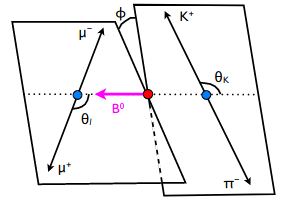
\includegraphics[width=0.5\textwidth]{flavor_plots/angular_describtion.png}
  \caption{image of the angular observables.\cite{Chatrchyan:2013cda}}
  \label{fig:angle_1}
\end{figure}

In this analysis, the forward-backard asymmetry $A_{FB}$, $F_L$ the fraction of the longitudinal polarisation of the $K^{*0}$ and the decay rate of the process $B^0 \to K^{*0} \mu \mu$ was measured. The definition of the angular observables are the following.
$\theta_{l}$ is the angle between the negatively charged lepton and  $\bar{B}$ in the dimuon center of mass system (c.m.s).
$\theta_{k}$ is the angle between the Kaon and the $\bar{B}$ in the $K^{*0}$ c.m.s..
The angle between the $K^{*0}$-plane and the dimuon-plane is defined by the angle $\phi$\cite{Bobeth:2010wg}.

Considering that S-wave contribution, spinless $K^{+}\pi^{-}$ constellations, can pollute the measurement, therfore a parametrization such as $\left(1 - F_S\right)$ for this was taken into account where $(1 -F_S)$ is the S-wave fraction which describes the amount of S-wave contribution.
The interference Amplitude between P-wave and S-wave decays are parametrized by $A_S$.
The angular distribution\cite{Chatrchyan:2013cda} for the $B^0 \to K^{*0} \mu \mu$ decay reads
\begin{equation*}
  \frac{1}{\Gamma}\frac{\symup{d}^3\Gamma}{\symup{d}\theta_k\symup{d}\theta_l\symup{d}q^2} = f\left(F_S, A_S, \theta_k, \theta_l, A_{FB}, F_L\right)
\end{equation*}
Since $A_{FB}$, $F_L$ and $\mathcal{A}\times\Epsilon$ do not depend on the angle $\phi$, it is already integrated out.
The angular description for The $B$ and $\bar{B}$ are combined afterwards and expanded into a sum of the angular variables multiplied with a fitparameter, which are the $A_{FB}$, $F_L$ and $S_i$\ref{fig:dubgamma}, which are called CP-averaged observables because they contain CP violation.

\begin{figure}[htb]
  \centering
  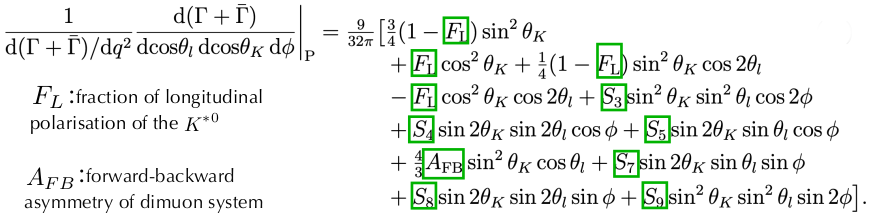
\includegraphics[width=0.5\textwidth]{flavor_plots/double_gamma.png}
  \caption{Angular description for $B$ and $\bar{B}$ combined.}
  \label{fig:dubgamma}
\end{figure}

Then the fit in the $S_i$ basis was reparametrised to the $P_i$ basis.
This was done to eliminate first order uncertainties in the form factors primarily.
The fit yields seven CP violating observables including $F_L$.
\begin{align*}
  P_1 &= \frac{2 S_3}{1 - F_L} & P_{4,5,8}\prime &= \frac{S_{4,5,8}}{\sqrt{F_L\left( 1 - F_L \right)}} \\
  P_2 &= \frac{2}{3}\frac{A_{FB}}{1 - F_L} &  P_6\prime &= \frac{S_7}{\sqrt{F_L\left( 1 - F_L \right)}} \\
  P_3 &= \frac{- S_9}{1 - F_L} \\
\end{align*}

This analysis especially focuses heavily on the tension induced by $P_5\prime$, since it is a very sensitive variable for $C_9$.
This can be seen in the range of $4$ - $8$ $\frac{\symup{GeV}}{c^4}$.
For every collaboration a discrepancy of between the SM and the measurement
displayed in figure \ref{p5tension}

\begin{figure}[htb]
  \centering
  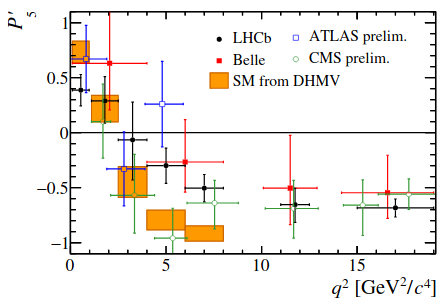
\includegraphics[width=0.5\textwidth]{flavor_plots/tension_in_p5.png}
  \caption{tension in $P_5\prime$.\cite{Blake:2017wjz}}
  \label{p5tension}
\end{figure}

% \section{early LHCb Measurementsand local tension}
Angular analysis for local tension in $P\prime_5$ performed by other collaborations such as ATLAS and CMS show similar results but Data taken stops at roughly the $J\/\Psi$ Mass due to the resonant background.
Therefore the ATLAS measurement is not so good.
As seen in some global fits, the shift in the wilson coefficent
$\text{Re}\left(C_9\right)$, the deviations in these wilson coefficents or up to $3$ - $5$ $\sigma$. In general, these fits are a good tool to learn from the fits.

% \section{the data set and Selection of Candidates}
The data used comes from the years 2011, 2012, which was Run 1, and 2016. The center of mass energies were 7, 8 and 13 $\si{\tera\electronvolt}$ respectively.
The data taken in the later years is nearly double from what the have taken in 2011.

For the stated process, it is required that the impact parameter for the daughters are quite large because they don't come from the primary vertex.
Also the PID\footnote{particle identification} is used to suppress the peaks in the background.
Machine learning algorithms are used to reduce combinatorial background.
For the probe regions in the $q^2$ plot, the signal regions muste be seperated fromm the background regions.
Since there are decay modes which have the same final state as our wanted process, there are several peak regios which muste be cut out. This is for example the charmonium background of the
$J\/\Psi$ and the $\psi$ meson.
The signal regions for the decay mode $b \to s \mu \mu$ can the be interpreted seperately. Also the photon pole at $q^2 = 0$. can be examined.

The binning used is historically conditioned. The only cause for that is to compact the data. One boundary at $\SI{1.1}{\giga\electronvolt}$ is set to delete the $\phi(1020)$ resonance from the data.

% \section{angular fit model}
To describe now the physics behind the angular analysis, instead of using the non-pertubative QCD form factors and the wilson coefficents, angular amplitudes $\symup{A}^{L\/R}$ are defined.
Then we measure in the bins of $q^2 = m^2(\mu \mu)$ by firstly integrating over $q^2$ and secondly combining this with the $B^0$ and $\bar{B}^0$ decays.
This results in a so called CP-averaged basis $S_i$.
The resulting $\frac{\symup{d}\Gamma}{\symup{d}q^2}$ spectrum is then
\begin{equation*}
  \frac{1}{\frac{\symup{d}\left(\Gamma + \bar{\Gamma}\right)}{\symup{d}q^2}} \cdot
  \frac{\symup{d}\left(\Gamma + \bar{\Gamma}\right)}{\symup{d}\cos\theta_l\symup{d}\cos\theta_k\symup{d}\phi}
  \rvert_P = \frac{9}{32\pi}\cdot f(F_{L}, \theta_{k}, \theta_{l}, A_{FB}, S_{i})
\end{equation*}

Here, the $F_L$ describes the fraction of longitudinal polarisation of the $K^{0*}$. $A_{FB}$ ist the forward/backward asymmetry of the dimuon system.
In order the reduce uncertainties, the first basis of the $S_i$ is transformed into a basis $P_i$ which takes ratios of observables\cite{cern}.

% \section{full fit model}
In the full fit model the shape of the invariant mass plots are used to determine the amount of signal and background in the data.
\begin{equation*}
  \symup{PDF}_{total} = f_{sig}\symup{PDF}_{sig}(\vec{\Omega}, m) +
  (1 - f_{sig})\symup{PDF}_{bkg}
\end{equation*}

The PDF function can be separated into an angular part and a massive part.
After that a maximum likelihood fit is performed.
As seen in figure \ref{fig:fullfit} the massive part of the signal PDF is a gaussian fucntion with a radiative tail and the background PDF results in a exponential function.

\begin{figure}[htb]
  \centering
  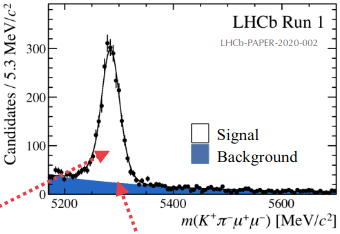
\includegraphics[width=0.5\textwidth]{pictures/fullfit.png}
  \caption{invariant B mass of Run 1 LHCb data.}
  \label{fig:fullfit}
\end{figure}

Because of the factorization of the signal and background PDF
\begin{equation*}
  \symup{PDF}_{sig}(\vec{\Omega}, m) = \symup{PDF}_{sig}(\vec{\Omega}) \times \symup{PDF}_{sig}(m)
\end{equation*}
the angular part of the signal PDF of the Run 1 data and the data from 2016 can be shared in the analysis to perform a simultaneous fit $\sum_I S_{i, q_{bin}^2} f_i(\Omega)$.

% \section{modelling the efficiencies}
Because the angular distribution and the $q^2$ distribution are influenced by the efficiencies, the parametrisation must be well known.
This is done via an acceptance function, her the legendre polynomials. With 3 angles and $q^2$ a 4D parametrisation results in 4 coefficents

% \section{s-wave contribution}
The $K \pi$ final state has more than one spin eigenstate. Therefore, additional terms are needed to differentiate between these states.
Because $K \pi \mu \mu$ can be produced in a vector state which disturbs the angular distribution, the different structures of the spin 1 $K^{0*}$ and the flat structure of the $K \pi$ state need to be analyzed.

% \section{uncertainties}
The dominant systematic uncertainties across the $q^2$ bins are acceptance variation with $q^2$, peaking backgrounds and the bias correction.
The whole table of uncertainties is shown in figure \ref{fig:unc}\cite{cern}.
\begin{figure}[htb]
  \centering
  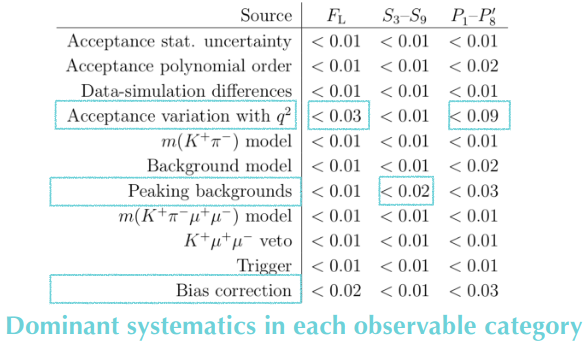
\includegraphics[width=0.5\textwidth]{pictures/uncertainties.png}
  \caption{table of systematic uncertainties.}
  \label{fig:unc}
\end{figure}

Because of different decays in the same target finalstate, for example $\bar{\Lambda}_b^0 \to \bar{p} \to \pi^{-} K^{+} \mu \mu$, events that are drawn from distributions of these peaking backgrounds are not taken into the fit.
Bias corrections come up if boundary effects like $F_S > 0$ are required.
\begin{equation*}
  ~\frac{\symup{d}\Gamma}{\symup{d}q^2}\rvert_{S + P} = \left(1 - F_S \right) ~\frac{\symup{d}\Gamma}{\symup{d}q^2}\rvert_P
\end{equation*}
For small $F_S$ the bias towards higher values biases the P-wave and vice versa.

% \section{Results and conclusion}
If the energy threshold is so big, that a $c\bar{c}$ pair can be produced in a loop which generates a $J \/ \Psi$, the would be a possibility to detect it.

The tension is confirmed with the 2016 data set.
The significance of the discrepancy is nuisance parameter dependend and also depends on the $q^2$ bins.
\printbibliography{}
\end{document}
